\documentclass[12pt]{article}
\usepackage{amsmath,amssymb}
\usepackage{mathrsfs}
\usepackage[mathscr]{euscript}
\usepackage{bbold}
\usepackage{esvect}
\usepackage{amsfonts}
\usepackage{cancel}
\usepackage{tikz-feynman}
\linespread{1}

\begin{document}
 


\title{From UV to Relativistic EFT}
\author{Puwen Sun}
\date{}
\maketitle


\section{From UV to Relativistic EFT}



The neutral components of scalar doublet or fermion-like doublet serve as the dark matter candidate. Both candidates interact with nucleons in direct detection through quarks and not gluons at leading order. 
Both scalar and fermionic SU(2) electroweak doublet, at leading order, interact via T-channel Z boson exchange. The momentum dependence enters through several places, including S-matrix elements and form factors. 
The DM-SM particle scattering via Z boson exchange will be matched into a general relativistic effective theory describing dark matter interactions with quarks and gluons. We will see that a lot of the Wilson coefficients will be zero in our case. But the steps here demonstrated the general procedures. The Wilson coefficients will be found through matching of the coefficients. The Wilson coefficients obtained can be passed to the next section as inputs for further calculations. 


\subsection{scalar doublet}
The scalar doublet dark matter interact weakly in direct detection experiment, at tree level, through Z boson exchange from gauge couplings. 
The kinetic term in Lagrangian with covariant derivatives are 
$$
\mathcal L = D_\mu \chi ^\dagger D^\mu \chi + ...
$$
expanding with $\chi = ( \chi^+ \chi^0 )^T $and using only electroweak gauge 
$D_\mu = \partial_\mu + ig_2 A_\mu^a T^a + ig_1 Y B_\mu $
gives
\begin{equation}
\begin{aligned}
 D_\mu \chi ^\dagger D^\mu \chi 
 &= [(\partial_\mu + ig_2 A_\mu^a T^a + ig_1 Y B_\mu) \begin{pmatrix}
\chi^+  \\   
\chi^0
\end{pmatrix}
]^ \dagger
 (\partial_\mu + ig_2 A_\mu^a T^a + ig_1 Y B_\mu) \begin{pmatrix}
\chi^+  \\ \chi^0
\end{pmatrix}\\
&= i  \frac{g_2}{2\cos \theta_w}\chi^{0*} Z_\mu (\partial^\mu \chi^0 ) - i  \frac{g_2}{2\cos\theta_w} (\partial^\mu \chi^0 )^*Z_\mu ( \chi^0 ) + ...
\end{aligned}
\end{equation}
where the value of hyper-charge was evaluated at $Y=\frac{1}{2}$, a is $SU(2) \times U(1) $ generator indices, and we ignored all irrelevant terms for this calculation in the .... 
For this calculation, we only need to know the the Feynman rule for the neutral component scalar doublet propagators are the same as that for a complex scalar field $\phi$. 
\begin{center}
\begin{tikzpicture}
  \begin{feynman}
    \vertex (a1) ;
    \vertex[right=1.5cm of a1] (a2);
    \diagram* {
      (a1) -- [charged scalar] (a2),
    };
  \end{feynman}
  \end{tikzpicture}
$= \frac{i}{p^2 - m^2 +i \epsilon}$ 
\end{center}
and the Feynman rule for the interactions between Z boson and neutral scalar field is 
\begin{center}
\begin{tikzpicture}
  \begin{feynman}
    \vertex (a1) ;
    \vertex[below=0.5cm of a1] (a2);
     \vertex at ($(a1) + (0.5cm,0.5cm)$)(a3);
    \vertex at ($(a1) + (-0.5cm,0.5cm)$) (a4);
    \diagram* {
      (a1) -- [ boson] (a2),
            (a1) -- [ scalar] (a3),
      (a1) -- [ scalar] (a4),
    };
  \end{feynman}
  \end{tikzpicture}
$= - i g_2' (p+p')^\mu$
\end{center}
where $g_2' $ can be read-off from above as $g_2 / 2\cos \theta_w$. The momentum of incoming scalar and outgoing scalar field is due to the derivatives.  

The Feynman rule for Z boson scattering with quarks is the Standard Model fermion coupling. 
The chiral structures are put into the coefficients $c_V$ and $c_A$ so that we do not need to write them explicitly every time. 
Since we only care about the Z boson, we only write
$$
\mathcal L = g_2 Z_\mu^0 J_Z^\mu  + ...
$$
where 
\begin{equation}
\begin{aligned}
 J_Z^\mu   = \frac{1}{\cos\theta_W} [ ... 
 &+ \bar u_L \gamma^\mu (\frac{1}{2} - \frac{2}{3} \sin^2 \theta_W ) u_L 
+ \bar u_R \gamma^\mu ( \frac{2}{3} \sin^2 \theta_W ) u_R \\
& + \bar d_L \gamma^\mu (\frac{1}{2} + \frac{1}{3} \sin^2 \theta_W ) d_L 
 + \bar d_R \gamma^\mu ( \frac{1}{3} \sin^2 \theta_W ) d_R + ...
 \end{aligned}
 \end{equation}
 where all other gauge couplings and all other terms inside Z neutral current from Standard Model are implied but not written down explicitly. The same is true for second and third generations of quarks. 
 I will use $c_V^q$ to represent the coefficient of the vector current part $\bar q \gamma_\mu q$ and $c_A^q$ to represent the coefficient of the axial vector current part $\bar q \gamma_\mu \gamma_5 q$ for a particular quark type.  
 For example
 \begin{equation}
 \begin{aligned}
 c_V^u 
 &
 = \frac{1}{2 }(\frac{1}{2} - \frac{2}{3} \sin^2 \theta_W ) +  \frac{1}{2}( \frac{2}{3} \sin^2 \theta_W )\\
 &= \frac{1}{4}
 \end{aligned}
  \end{equation}
  \begin{equation}
 \begin{aligned} c_A^u 
 &= - \frac{1}{2}(\frac{1}{2} - \frac{2}{3} \sin^2 \theta_W ) +  \frac{1}{2}( \frac{2}{3} \sin^2 \theta_W )\\
 &= - \frac{1}{4} + \frac{2}{3} \sin^2 \theta_W 
 \end{aligned}
   \end{equation}
The Feynman diagram

\begin{center}
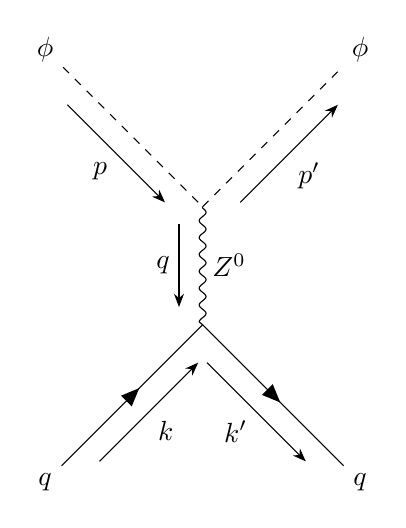
\begin{tikzpicture}
  \begin{feynman}
    \vertex (a1) ;
    \vertex[below=1.5cm of a1] (a2);
    \vertex at ($(a1) + (2cm, 2cm)$) (b2){\( \phi \)};
    \vertex at ($(a1) + (-2cm, 2cm)$) (b1){\( \phi \)};
    \vertex at ($(a2) + (-2cm, -2cm)$) (c2){\( q \)};
    \vertex at ($(a2) + (2cm, -2cm)$) (c1){\( q \)};

    \diagram* {
        (c2) --[ fermion, momentum'=\(k\)] (a2) --[ fermion, momentum'=\(k'\)] (c1),
      (a1) -- [boson, edge label=\(Z^0\), momentum'=\(q\)] (a2),
      (b1) --[scalar, momentum'=\(p\)] (a1) -- [scalar, momentum'=\(p'\)] (b2),
    };
  \end{feynman}
\end{tikzpicture}
\end{center}

can now be evaluated 
$$
= [- i g_2' P^\mu][ - i\frac{g_2}{\cos \theta_W}  c_L^q] [\frac{-i g_{\mu\nu}+i \frac{q_\mu q_\nu }{m_Z^2} }{q^2-m_Z^2 + i\epsilon } ] [\bar u_{S'}(k')   \gamma^\nu  (\frac{1-\gamma_5}{2}) u_S(k)]
$$
where $c_L^q$ is the coupling coefficient between Z boson and left-handed quark, equal to either $ (\frac{1}{2} - \frac{2}{3} \sin^2 \theta_W)$ or $ (\frac{1}{2} + \frac{1}{3} \sin^2 \theta_W)$depending on whether it is up-type or down-type, and $P^\mu =( p+p')^\mu$ is the sum of the initial and final four-momentum of scalar particle, q is the four-momentum of Z intermediate Z boson, and S and S' are the spin state of the initial and final quarks. This is for left-handed quarks while similar structure for right handed ones, replacing $c_L^q$with $c^q_R$ and $(1- \gamma_5)/2$ with $(1+\gamma_5)/2$. The square S-matrix element is then proportional to the spin sum of the above Feynman amplitude
\begin{equation}
\begin{aligned}
\frac{1}{2}\sum_{S,S'} \mid \mathcal M \mid ^2 = 
&
\frac{1}{2} g_2 ^{'2} \frac{g_2^2}{\cos^2 \theta_W} c^{q2}_L \frac{P^\mu P^\nu - 4(P \cdot q ) P^{(\mu} q^{\nu)} / m_Z^2 + (P \cdot q )^2 q^\mu q^\nu / m_Z^4 }{(q^2-m_Z^2 +i\epsilon)^2} \\
 &  Tr[(\cancel k'+m_q)  \gamma_\mu (\cancel k+m_q) \gamma_\nu \frac{1-\gamma_5}{2}]
\end{aligned}
\end{equation}
where $(\mu \nu)$ means the symmetric part of it. Therefore, the above is followed by, using the traces identities, 

\begin{equation}
\begin{aligned}
\frac{1}{2}\sum_{S,S'} \mid \mathcal M \mid ^2 = 
&
 \frac{ g_2 ^{'2} g_2 ^2  c_L^{q2}}{(q^2-m_Z^2 +i\epsilon)^2\cos^2 \theta_W} 
  (2(k' \cdot P)(k \cdot P)-( k \cdot k' - m_q^2)(P \cdot P )\\
 &
 + i  \epsilon_{\mu\nu\rho\sigma} P^\nu P^\sigma k'^\mu k^\rho ) + ...
\end{aligned}
\end{equation}
where the dots mean that the terms are suppressed by $\frac{q^2}{m_Z^2}$ and this factor is small in dark matter direct detection. 

The above result is translated into a general relativistic effective theory which describes scalar dark matter interact with quarks. The full set of operators are discussed in section (). Here, the relevant operators are
$$
\mathcal Q_{1,q}^{(6)} = (\phi^* i \overleftrightarrow\partial_\mu \phi ) ( \bar f \gamma^\mu f ) 
$$
and 
$$
\mathcal Q_{1,q}^{(6)} = (\phi^* i \overleftrightarrow\partial_\mu \phi ) ( \bar f \gamma^\mu\gamma_5 f ) 
$$
where the arrow means $A \overleftrightarrow\partial B= (\partial A)B-A(\partial B)$. The translation is done by performing the matching of the Wilson coefficients, which can be $ \mathcal  C_{1,q}$ for the first one and $\mathcal  C_{2,q}$  for the second one. 
The square matrix element of the first effective operator is evaluated in a similar way, by finding the vertex factor of the four-vertex that scatter a general scalar field with a general fermion
\begin{center}
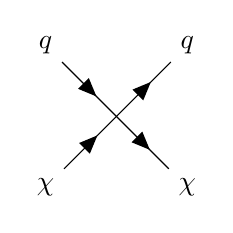
\begin{tikzpicture}
  \begin{feynman}
    \vertex (a1) ;
    \vertex  at ($(a1) + (0.9cm,-0.9cm)$)(a2){\( \chi \)};
       \vertex at   ($(a1) + (-0.9cm,-0.9cm)$)(a5){\( \chi \)};
     \vertex at ($(a1) + (0.9cm,0.9cm)$)(a3){\( q \)};
    \vertex at ($(a1) + (-0.9cm,0.9cm)$) (a4){\( q \)};
    \diagram* {
      (a1) -- [ fermion] (a2),
            (a5) -- [ fermion] (a1),
            (a1) -- [ fermion] (a3),
      (a4) -- [ fermion] (a1),
    };
  \end{feynman}
  \end{tikzpicture}
$= -i  \mathcal C^{(6)}_{1,q} (p+p')^\mu$
\end{center}
which in turn leads to the matrix element
\begin{center}
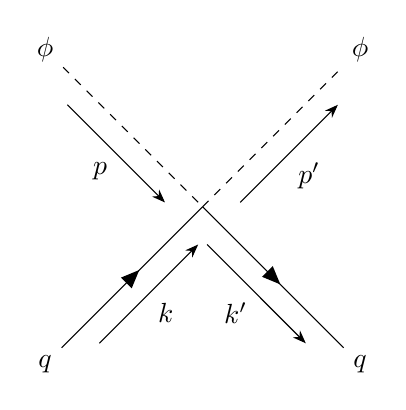
\begin{tikzpicture}
  \begin{feynman}
    \vertex (a1) ;
    \vertex at ($(a1) + (2cm, 2cm)$) (b2){\( \phi \)};
    \vertex at ($(a1) + (-2cm, 2cm)$) (b1){\( \phi \)};
    \vertex at ($(a1) + (-2cm, -2cm)$) (c2){\( q \)};
    \vertex at ($(a1) + (2cm, -2cm)$) (c1){\( q \)};
    \diagram* {
        (c2) --[ fermion, momentum'=\(k\)] (a1) --[ fermion, momentum'=\(k'\)] (c1),
      (b1) --[scalar, momentum'=\(p\)] (a1) -- [scalar, momentum'=\(p'\)] (b2),
    };
  \end{feynman}
\end{tikzpicture}
\end{center}
$$
\mid \mathcal  M \mid^2 = \mid \mathcal  C_{1,q}^{(6)}  \mid^2 P_\mu P_\nu  [\bar u_{S'}(k')   \gamma^\mu  u_S(k)] [\bar u_{S}(k)   \gamma^\nu   u_{S'}(k')]
$$
where P also means $p+p'$ here. The spin sum then gives
$$
\frac{1}{2}\sum_{S,S'} \mid \mathcal M \mid ^2 = 
 \mid \mathcal  C_{1,q}^{(6)}  \mid^2 P_\mu P_\nu Tr[(\cancel k'+m_q)  \gamma_\mu (\cancel k+m_q) \gamma_\nu]
$$
contracting Lorentz indices gives
$$
\frac{1}{2}\sum_{S,S'} \mid \mathcal M \mid ^2 =
2 \mid \mathcal  C_{1,q}^{(6)}  \mid^2 [ 2(k' \cdot P)(k \cdot P)-( k \cdot k' - m_q^2)(P \cdot P )]
$$
therefore, matching coefficient at leading order in the large $m_Z$ limit, 
\begin{equation}
\begin{aligned}
   \mathcal  C_{1,q}^{(6)} 
 &
=   \frac{1}{2} g_2' \frac{g_2}{\cos \theta_W}( c_L^{q}+c_R^{q}) \frac{1}{m_Z^2}\\
& = \frac{g_2^2 ( c_L^{q}+c_R^{q}) }{4\cos^2\theta_Wm_Z^2}\\
&= 2\sqrt 2 G_F c_V
 \end{aligned}
 \end{equation}
 similarly, 
 $$
 \mathcal  C_{2,q}^{(6)}  = 2\sqrt 2 G_F c_A
$$

\subsection{fermion doublet}
The leading order Z boson exchange of fermion dark matter $\psi$ with the vector and axial vector current is calculated and matched in a similar way. The kinetic term in Lagrangian with electroweak covariant derivative are
$$
\mathcal L = i \bar \psi \cancel D \psi + ...
$$
where the fermion doublet is $\psi = ( \psi_{DM} , \psi^-)$ and covariant derivative here also only includes the weak gauge.  The hyper-charge is evaluated at $Y=-\frac{1}{2} $ for fermion doublet. The terms relevant for Z boson exchange between DM and SM quarks are just 
$$
i  \bar \psi \cancel D \psi  = i \frac{g_2}{2\cos \theta_W}  \bar \psi_{DM} Z_\mu \psi_{DM} + ...
$$
This is just similar to the SM weak interactions of SM fermions. The vertex Feynman rule is given by
\begin{center}
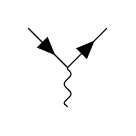
\begin{tikzpicture}
  \begin{feynman}
 \vertex (a1) ;
    \vertex[below=0.5cm of a1] (a2);
     \vertex at ($(a1) + (0.5cm,0.5cm)$)(a3);
    \vertex at ($(a1) + (-0.5cm,0.5cm)$) (a4);
    \diagram* {
      (a1) -- [ boson] (a2),
            (a1) -- [ fermion] (a3),
      (a4) -- [ fermion] (a1),
    };
  \end{feynman}
\end{tikzpicture}
$= - i\frac{ g_2 }{2 \cos \theta_W}  $
\end{center}
and the external fermion dark matter follows the same rule as the SM fermions. 
Therefore, the effective theory vertex of the DM-SM scattering is just a 4-Fermi like vertex proportional to the Fermi constant $G_F$. 

 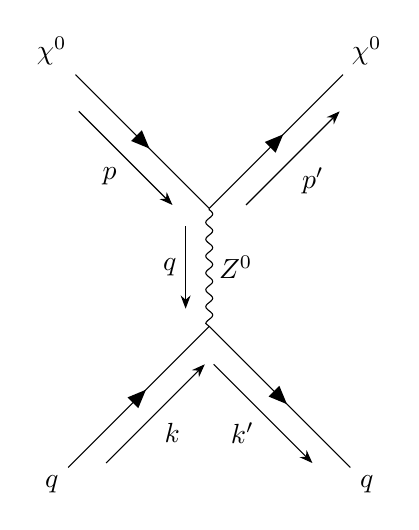
\begin{tikzpicture}
  \begin{feynman}
    \vertex (a1) ;
    \vertex[below=1.5cm of a1] (a2);
    \vertex at ($(a1) + (2cm, 2cm)$) (b2){\( \chi^0 \)};
    \vertex at ($(a1) + (-2cm, 2cm)$) (b1){\( \chi^0 \)};
    \vertex at ($(a2) + (-2cm, -2cm)$) (c2){\( q \)};
    \vertex at ($(a2) + (2cm, -2cm)$) (c1){\( q \)};
    \diagram* {
        (c2) --[ fermion, momentum'=\(k\)] (a2) --[ fermion, momentum'=\(k'\)] (c1),
      (a1) -- [boson, edge label=\(Z^0\), momentum'=\(q\)] (a2),
      (b1) --[fermion, momentum'=\(p\)] (a1) -- [fermion, momentum'=\(p'\)] (b2),
    };
  \end{feynman}
\end{tikzpicture}

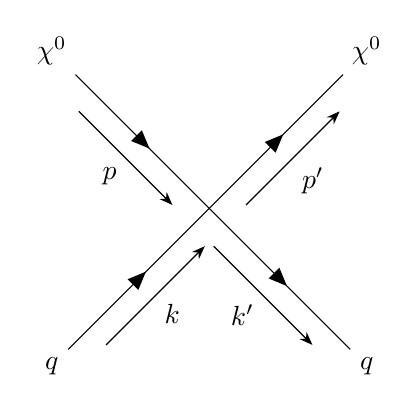
\begin{tikzpicture}
  \begin{feynman}
    \vertex (a1) ;
    \vertex at ($(a1) + (2cm, 2cm)$) (b2){\( \chi^0 \)};
    \vertex at ($(a1) + (-2cm, 2cm)$) (b1){\( \chi^0 \)};
    \vertex at ($(a1) + (-2cm, -2cm)$) (c2){\( q \)};
    \vertex at ($(a1) + (2cm, -2cm)$) (c1){\( q \)};
    \diagram* {
        (c2) --[ fermion, momentum'=\(k\)] (a1) --[ fermion, momentum'=\(k'\)] (c1),
      (b1) --[fermion, momentum'=\(p\)] (a1) -- [fermion, momentum'=\(p'\)] (b2),
    };
  \end{feynman}
\end{tikzpicture}

Following the above method, the relevant relativistic effective operators describing fermionic dark matter scattering with SM quarks are presented here, while a complete set are presented in the later sections for a more general discussion. The relevant operators here are
$$
  \mathcal Q_1^{(6)} = (\bar \chi \gamma_\mu \chi ) (\bar q \gamma^\mu q)
$$
$$
  \mathcal Q_3^{(6)} = (\bar \chi \gamma_\mu \chi ) (\bar q \gamma^\mu \gamma_5 q)
$$
The Wilson coefficients can be read-off from above
\begin{equation}
\begin{aligned}
\mathcal C_{1,q}^{(6)}
&
= \frac{g_2}{2 \cos \theta_W } \frac{1}{m_Z^2} \frac{g_2 c_V^q}{\cos \theta_W}\\
& = 2\sqrt 2 G_F c_V^q
\end{aligned}
\end{equation}
\begin{equation}
\begin{aligned}
\mathcal C_{3,q}^{(6)}
&
= \frac{g_2}{2 \cos \theta_W } \frac{1}{m_Z^2} \frac{g_2 c_V^q}{\cos \theta_W}\\
& = 2\sqrt 2 G_F c_A^q
\end{aligned}
\end{equation}
This section shows explicitly that how Z boson is integrated out to match the UV theory into a relativistic EFT, which provides the basis for the calculation of event rates of scalar or fermion dark matter scattering with nucleus in the later sections. 









\end{document}






